\documentclass[sigconf,review]{acmart}

\usepackage{amsmath,amssymb,amsfonts,latexsym}
\usepackage{enumerate}
\usepackage{xspace}
\usepackage{epsf,picinpar}
\usepackage{varioref}
\usepackage{colortbl,multirow,hhline}
\usepackage{listings}
\usepackage{amssymb}
\usepackage{colortbl,multirow,hhline}
\usepackage{algorithmic}
\usepackage{algorithm}
\usepackage{caption}
\usepackage[normalem]{ulem}
\usepackage{xcolor}
\usepackage{pifont}
\usepackage{xcolor,colortbl}
\usepackage{url}
\usepackage{balance}
\usepackage{graphicx, subfigure}
\usepackage{longtable}
\usepackage{lscape}
\usepackage{multirow}
\usepackage{listings}
\usepackage{framed}
\usepackage{morefloats}
\usepackage[T1]{fontenc}
\usepackage{array}
\usepackage{pdfpages}
\usepackage{fancybox}
\usepackage{amsmath}
\usepackage{flushend}
\usepackage{booktabs}
\usepackage{enumitem}
\usepackage[acronym]{glossaries}
\usepackage{wrapfig}

% \usepackage[table]{xcolor}


\renewcommand{\ttdefault}{cmr}

%\newcommand{\limit}[1]{\textcolor{red}{\noindent \ding{46}~Page limit:~#1}\\}
\newcommand{\todo}[1]{\textcolor{red}{\ding{46}~#1}} 
\newcommand{\ie}{\emph{i.e.,}\xspace}
\newcommand{\eg}{\emph{e.g.,}\xspace}
\newcommand{\etc}{etc.\xspace}
\newcommand{\etal}{\emph{et~al.}\xspace} 

%%% ----- ACRONYMS ----- %%%
\makeglossaries
\newacronym{plt}{PLT}{Page Load Time}
\newacronym{js}{JS}{JavaScript}
\newacronym{pwas}{PWAs}{Progressive Web Applications}
\newacronym{pwa}{PWA}{Progressive Web Application}

\copyrightyear{2020}
\acmYear{2020}
\setcopyright{acmcopyright}
\acmConference[Green Lab 2020/2021]{Green Lab 2020/2021 - Vrije Universiteit Amsterdam}{September--October, 2020}{Amsterdam, The Netherlands}
\acmBooktitle{Green Lab 2020/2021 - Vrije Universiteit Amsterdam, September--October, 2020, Amsterdam (The Netherlands)}
    
\begin{document}

\title{
	The Impact of Cluttered JavaScript Code in Mobile Web Apps with respect to Energy Consumption
}


\author{Geoffrey van Driessel}
\affiliation{%
 \institution{2639310 \\ VU Amsterdam}
} \email{g.r.van.driessel@student.vu.nl}

\author{Abijith Radhakrishnan}
\affiliation{%
 \institution{2667575 \\ VU Amsterdam}
} \email{a.radhakrishnan@student.vu.nl}

\author{Sophie Vos}
\affiliation{%
 \institution{2551583 \\ VU Amsterdam}
} \email{s.o.vos@student.vu.nl}

\author{Marc Wiggerman}
\affiliation{%
 \institution{2653796 \\ VU Amsterdam}
} \email{m.g.wiggerman@student.vu.nl}

% \author{Name Surname}
% \affiliation{%
%  \institution{Student Number \\ VU Amsterdam}
% } \email{xyz@student.vu.nl}

\begin{abstract}
\noindent \textit{Context}. 
Mobile phones are a major contributor to global internet traffic. Although, the energy usage of a single smartphone may be considered modest, the overall energy footprint left by mobile devices is far higher. Thiagarajan et al.~\cite{thiagarajan2012battery}, showed that JavaScript (JS) code mainly contributes to the energy consumption relative to other web elements. Chaqfeh et al.\cite{chaqfeh2020jscleaner}~introduced a tool, called \textit{JSCleaner}, that de-clutters mobile web apps by removing non-essential JS code. They showed that this positively influences the Page Load Time. 

\noindent \textit{Goal}. 
Since energy-efficiency contributes to the user experience and the environmental impact of increasingly popular mobile web apps, we aim to contribute by investigating the impact of cluttered JS code on energy consumption. The goal of our study is: ``Analyze cluttered JS code for the purpose of evaluation with respect to the energy consumption from the point of view of software developers in the context of mobile web apps".

\noindent \textit{Method}. 
To accomplish this goal, we conducted an empirical experiment to measure and compare the energy consumption of cluttered and de-cluttered mobile web apps. We randomly selected 27 diverse, currently operational mobile web apps as subjects. Furthermore, we used Android Runner and the Batterystats profiler to measure the energy consumption. 

\noindent \textit{Results}. We tested the energy consumption for small, medium, and large mobile web apps. Our results showed that cluttered mobile web apps do not influence the energy consumption. 

\noindent \textit{Conclusions}. Hence, based on this experiment, we do not recommend developers who aim to reduce the energy consumption of their mobile web app to apply a de-cluttering engine. It should be noted that we tested the difference in energy consumption using a relatively small dataset and using a single de-cluttering engine. Therefore, further research is required to support this claim.
\end{abstract}

\maketitle

\section{Introduction}
% This document represents a template of the final experiment report structure for the course \textit{Green Lab} at the Vrije Universiteit Amsterdam \cite{greenlab}.

% The experiment is conducted according to the guidelines by Wohlin and colleagues \cite{wohlin12}.

% The total length of this document must not exceed 15 pages, including references, appendixes, \etc

% In this section you have to describe (i) the domain (\eg mobile apps and their market) and the technologies relevant for understanding the rest of the document, (ii) the main motivation behind your experiment (the problem, here you can show examples via apps/tools screenshots, snippets of source code, \etc), (iii) what your experiment is about (hint of the solution), and (iii) what the developers will learn from the results of your experiment.  

%%% ----- MOBILE TRAFFIC ----- %%%
CISCO predicted global internet traffic in 2020 to be equivalent to 95x the volume of the entire global internet in 2005 \cite{ciscoforecast}. Since the end of the second quarter of 2020, mobile devices (excluding tablets) have been a major contributor to global internet traffic. It accounts for 51.53\% of global website traffic and has an ascending trend. Corresponding to the increased traffic, the complexity of modern web pages has considerably advanced in the previous decade, leading to bigger web pages that are computationally intense for mobile devices. 

%%% ----- JS COMPLEXITY ----- %%%
The extended complexity in websites can be mainly attributed to the inception of web and \acrfull{js} frameworks (such as jQuery, Angular, React) \cite{persson2020javascript} which provide swift solutions for web development with function-specific modules and libraries that can fast pace the programming process. The debut of Single Page Applications (SPAs) further paved the way for more frameworks and standardization of web development. Nevertheless, this also led to \acrshort{js} files in websites being bloated with unused and unnecessary functions from the frameworks and ergo higher computational complexity.

%%% ----- MOBILE TRAFFIC & JS COMPLEXITY EFFECTS -> ENERGY & PLT ----- %%%
A computationally intensive website leads to higher energy consumption as well as increased \acrfull{plt}. It has been shown that web pages that have a \acrshort{plt} higher than 3 seconds, have a probability of losing 32\% of its visitors \cite{googlemobbench}. 
Even if the energy usage of a single smartphone may be considered modest, the overall energy footprint left by mobile devices is far higher \cite{timeenergy}. This was further extended by top-end smartphones and 4G network \cite{chen2014demystifying}. Google handled this by using lighter variants of web pages through Accelerated Mobile Pages (AMP). Another approach for reducing \acrshort{plt} commonly used by web developers is concatenation, minification, and uglification of different \acrshort{js} files in the web page. Even though this approach provides a slightly faster \acrshort{plt} because of smaller file size \cite{improvewebspeed}, \acrshort{js} computations in the browser remain the same. Furthermore, social media websites such as Facebook offers a lighter version of their service (Facebook Lite) which is better suited for low-power devices and more energy efficient.

%%% ----- RELEVANCE & SETUP OUR STUDY ----- %%%
% Our energy analysis
% its relevance
% importance
% motivation for the experiment
Another method to reduce PLT by reducing the amount of \acrshort{js} code is introduced by Chaqfeh et al.~\cite{chaqfeh2020jscleaner}. Chaqfeh et al.~\cite{chaqfeh2020jscleaner} introduced \textit{JSCleaner}: a classification algorithm that classifies critical, replaceable, and non-critical \acrshort{js} code. Accordingly, the replaceable \acrshort{js} code is replaced with HTML counterparts, and non-critical \acrshort{js} code is eliminated. This process is referred to as `de-cluttering'. The authors studied the relation between the de-cluttered web pages and the \acrshort{plt}. They concluded that de-cluttering achieves a 30\% reduction in \acrshort{plt}. A different study, conducted by Thiagarajan et al.~\cite{thiagarajan2012battery} showed that \acrshort{js} code has a relatively high energy consumption compared to other web elements. Since energy-efficiency contributes to the user experience and impact of increasingly popular mobile web pages, we aim to contribute by investigating the impact of eliminating \acrshort{js} code on energy consumption. Our research focuses on the relation between de-cluttered \acrshort{js} code using \textit{JSCleaner} on mobile web pages and its impact on energy consumption. Hence, our research question is: ``\textit{What is the impact of de-cluttering JavaScript code in mobile web pages using \textit{JScleaner} with respect to the energy consumption?}''.

%%% ----- EXPERIMENT DETAILS & PAPER STRUCTURE ----- %%%
% how will we answer the research question?

The remainder of this paper is structured as follows. Section 2 provides an insight into related work, and how this paper is compared to these related works. Next, section 3 defines the experiment using the GQM method. 

%\textcolor{red}{Page limit: 2}
% In this section, we describe the scientific papers similar to our experiment, both in terms of goal and methodology. 

% One paragraph for each paper (we expect about 5-8 papers to be discussed). Each paragraph contains: (i) a brief description of the related paper and (ii) a black-on-white description about how your experiment differs from the related paper.

\section{Related Work}\label{sec:related}

% An Extensible Approach for Taming the Challenges of JavaScript Dead Code Elimination
% http://www.ivanomalavolta.com/files/papers/SANER_2018.pdf
To the best of our knowledge, this paper is the first one to analyze and compare the energy consumption of mobile web apps using (1) the cluttered \acrshort{js} code base, and (2) the de-cluttered \acrshort{js} code base. Most of the research up until now focused on improving and analyzing the performance increase with relation to the \acrshort{plt}. First, we describe the work of Obbink et al.~\cite{Lacuna}, who introduced a tool called \textit{Lacuna}. Lacuna automatically eliminates dead \acrshort{js} code from mobile web apps, which in effect improves the \acrshort{plt} and energy consumption by reducing the required network and browser interpretation time. Obbink et al.~\cite{Lacuna} apply different analysis techniques to discover and eliminate dead code from the code base without changing the features of the mobile web app. After testing Lacuna on 29 mobile web apps, the results showed that Lacuna could be integrated into real-world build systems due to its reasonable execution time. 

%JSCleaner
Second, Chaqfeh et al.~\cite{chaqfeh2020jscleaner} present a way to automatically de-clutter \acrshort{js} code using a tool called JSCleaner. The proposed JS de-cluttering tool helps to reduce PLT in mobile web apps without significantly jeopardizing its content and functionality. It follows a rule-based classification algorithm that divides JS code into three classes: non-critical, replaceable, and critical. It then deletes non-critical JS code from the mobile web apps, interprets replaceable JS components with their corresponding HTML code, and maintains critical JS code without any modification. The study then quantitatively analyzed 500 popular mobile web apps and reports an empirical evaluation in which a 30\% reduction in \acrshort{plt} and a 50\% reduction in the number of requests and size using the JSCleaner tool is presented. A qualitative evaluation followed in which the authors recruited 103 users to analyze the difference in functionality between cluttered and de-cluttered mobile web apps. The de-cluttered mobile web apps maintained the appearance of the cluttered mobile web apps with a median value of over 93\%. Both papers \cite{Lacuna, chaqfeh2020jscleaner} introduce a different way to improve the \acrshort{plt}. However, they do not analyze the change in energy consumption of the cluttered versus the de-cluttered code base. 

Other studies perform a similar research methodology, only to accomplish a different goal. For example, Malavolta et al.~\cite{Evaluating_Caching} performed an experiment to test the performance and energy efficiency of \acrfull{pwas} while tuning the browser's cache behavior. The study involved measuring the energy consumption in joules and the \acrshort{plt} in milliseconds during the initial load of nine \acrshort{pwas} on a single Android device running in the Firefox browser. The authors concluded that the current results do not show evidence that adding caching to a website improves its energy efficiency. Despite the goal being different from the one presented in our study, the experimental setup and execution are similar to the ones presented in our study.

Another study that has a similar research methodology is the work of Chan-Jong-Chu~\cite{chan2020investigating}. The authors conducted an empirical experiment using mobile web apps with the aim to find a correlation between performance and energy consumption. The study has a clear research setup in which the correlation is proved using statistical tests together with a thorough description of the experiment execution. We provide a similar setup to ensure that the measured difference in energy consumption of cluttered and de-cluttered mobile web apps is statistically significant and the study can be precisely replicated.

% Who Killed My Battery:
% Analyzing Mobile Browser Energy Consumption
% http://crypto.stanford.edu/~dabo/pubs/papers/browserpower.pdf
Lastly, Thiagarajan et al.~\cite{thiagarajan2012battery} studied the energy consumption of downloading and rendering mobile web apps on mobile devices by comparing the different energy usage (in joules) of web elements. This is relevant to our research as we aim to understand the energy consumption of a specific modification in a mobile web app. Thiagarajan et al.~\cite{thiagarajan2012battery} aim to advise developers in designing energy-efficient mobile web apps. They concluded that the usage of \acrshort{js} code in mobile web apps has a negative effect on energy consumption compared to HTML elements. This is relevant to our study as we measure (a potential) energy gain by eliminating non-critical \acrshort{js} code or replacing the \acrshort{js} elements with HTML code. The main difference between the study of Thiagarajan et al.~\cite{thiagarajan2012battery} and our study is that the work of Thiagarajan et al. is more descriptive (they are trying to understand a phenomenon), whereas we aim at discovering a specific relationship (i.e., the one between being cluttered and consuming different amounts of energy).

%\textcolor{red}{Page limit: 1}
\section{Experiment Definition}

As described in the related work section, JSCleaner reduces the size of \acrshort{js} files significantly and, therefore, reduces the \acrshort{plt}. However, it has not been shown that this actually reduces the energy consumption. The \textbf{goal} of our study is: ``\textit{Analyze cluttered JavaScript code for the purpose of evaluation with respect to the energy consumption from the point of view of software developers in the context of mobile web apps}". This goal has been established using the GQM method ~\cite{claes2012experimentation}, the steps are presented in Table \ref{tab:goal}.

\begin{table}[H]
    \centering
    \begin{tabular}{||c || c||} 
     \hline
     Analyze & cluttered JavaScript code \\ 
     \hline
     For the purpose of & evaluating \\
     \hline
     With respect to the & energy consumption \\
     \hline
     From point of view of & software developers \\
     \hline
     In the context of & mobile web apps \\
     \hline
    \end{tabular}
    \caption{Goal}\label{tab:goal}
\end{table}

Following our goal, we have identified the \textbf{research question} \textbf{(RQ)}: ``\textit{What is the impact of cluttered JavaScript code in mobile web apps with respect to the energy consumption?}''. We answer this research question by comparing the energy consumption of popular mobile web pages compared to their de-cluttered version. The mobile web apps are de-cluttered by JSCleaner.

To answer our research question the energy consumption (in joules) is used as \textbf{metric}. The energy consumption is calculated using the measured \textit{power consumption (in watts)} times the \textit{\acrshort{plt} (in seconds)}. \textcolor{blue}{Furthermore, we measured the page size (in MBs) to block a potential effect of page size on the energy consumption.} 

\begin{figure}[H]
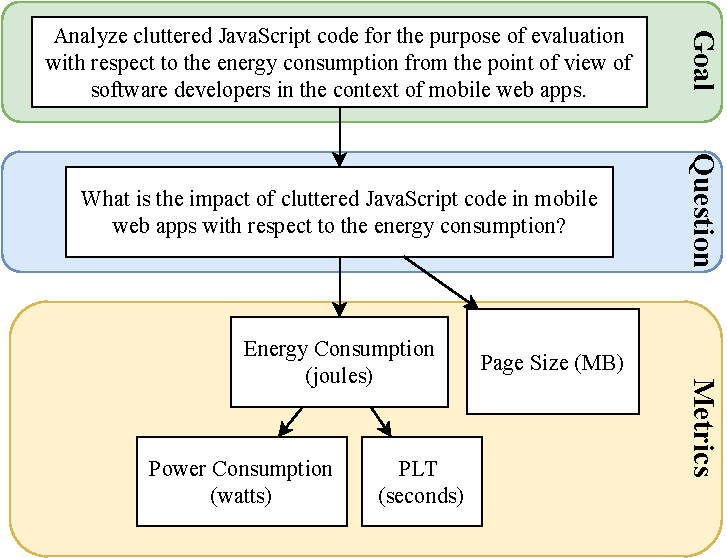
\includegraphics[width=8cm]{reportTemplate/figures/GQM.pdf}
\centering
\caption{The GQM Tree} \label{fig:gqm}
\end{figure}

Figure \ref{fig:gqm} presents a visual representation of the GQM. It hierarchically shows how the goal is obtained using the research question, and how the research question is answered using the metrics.
%\textcolor{red}{Page limit: 2}
\section{Experiment Planning}

\subsection{Subjects Selection}
\subsection{Experimental Variables}
\subsection{Experimental Hypotheses}
\subsection{Experiment Design}
% The evaluation will be done using the following method. A dataset containing 500 cluttered and 500 decluttered web pages will be used to sample a smaller set of webpages ${\sim}40$. 
% Then the first experiment will be to collect the energy consumption of loading the cluttered and decluttered web pages. Comparing this data will give an answer to our research question. An additional experiment will be to also measure the energy consumption of the decluttering process of JSCleaner. We can then 1) divide the energy consumption of the decluttering by the average amount of visitors per web page, then 2) add this to the energy consumption of loading the decluttered web page, and then 3) compare this again to the cluttered energy consumption.
\subsection{Data Analysis}

\textcolor{red}{Page limit: 3}
  
% Report about: how you plan to conduct your experiment, which tools you are going to use, which devices/laptops, figure and description of the overall software/hardware infrastructure you are setting up for the experiment (\eg who communicates with whom, proxies, network requests, order of actions, \etc).
%\textcolor{red}{Page limit: 2}

\section{Experiment Execution}\label{sec:experumnent_executuon}

In our experiment, we use an Android smartphone to load the mobile web apps. The smartphone used for the experiment is the \textcolor{blue}{Google Pixel 3 and has an octa-core (4x2.5 GHz Kryo 385 Gold and 4x1.6 GHz Kryo 385 Silver) processor with 4 GB of RAM}. This smartphone runs Android version 8.0.0. To mitigate the effects of background processes, we disable services we do not use such as Bluetooth, Location Services (GPS), and NFC. To ensure that the experiment stays running while minimizing the impact of the display on the measured energy consumption, the screen brightness is minimized while ensuring that the phone cannot go to sleep mode. Furthermore, we disabled all push notifications and non-critical apps. 

\begin{figure}[h]
\centering
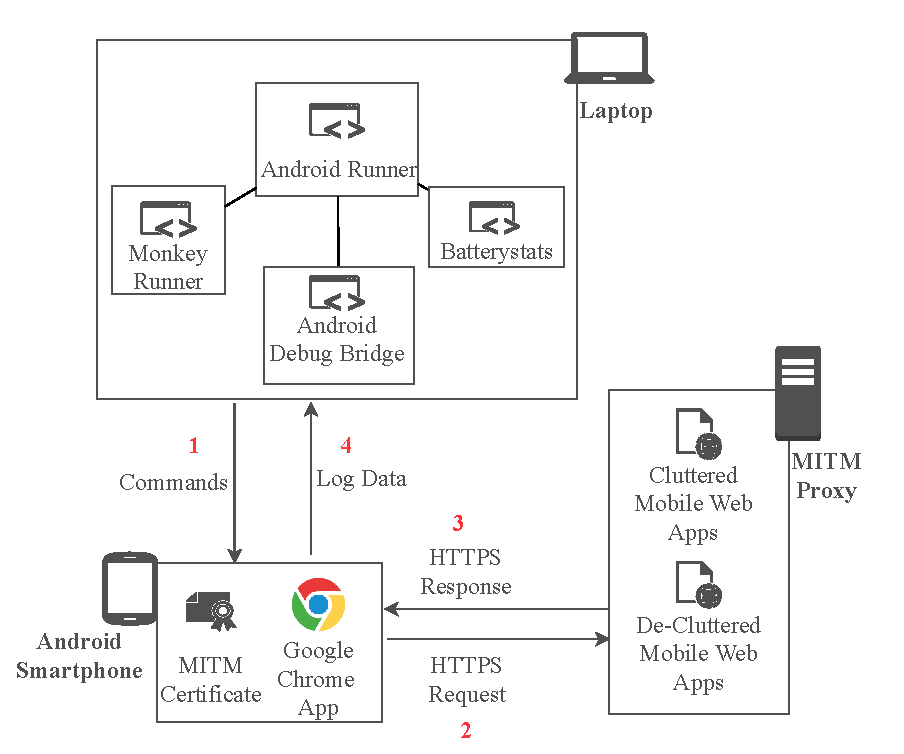
\includegraphics[width=9cm]{reportTemplate/figures/execution.pdf}
\caption{\textcolor{blue}{Experiment Execution}} \label{fig:deploymentview}
\end{figure}

The smartphone is connected to a laptop using Android Debug Bridge (adb)\footnote{\url{https://developer.android.com/studio/command-line/adb}}. The computer that we use to manage the experiment has an Intel i7 CPU (8th generation, 8 cores, and 4.2 GHz maximum clock speed) with 16 GB of RAM. Adb is a tool that allows communication between a development machine and an Android device. This communication entails information of the experiment configurations from the laptop to the smartphone and measurement data from the smartphone to the laptop. The Android smartphone and laptop are both connected to the same LAN. All the devices are in close proximity \textcolor{blue}{(less than a meter)} to the WiFi router (802.11ac standard and 5 GHz frequency band) to ensure minimum latency. The Android smartphone uses the Google Chrome web browser version \textcolor{blue}{{66.0.3359.158}} to access the internet and load the cluttered and de-cluttered mobile web apps. The researchers of the JSCleaner paper~\cite{chaqfeh2020jscleaner} cached the cluttered and de-cluttered mobile web apps, which they used for their research, on a proxy server and shared this proxy with us. In order to access the proxy server, the mitmproxy\footnote{\url{https://docs.mitmproxy.org/}} certificate \textcolor{blue}{is} installed on the smartphone. Mitmproxy is an HTTPS proxy that allows (among other features) interactive HTTPS requests. 

In order to \textcolor{blue}{execute} the experiment, we use Android Runner (AR)\footnote{\url{https://github.com/S2-group/android-runner}}. AR is a tool that facilitates the execution of measurement-based experiments on native apps and mobile web apps running on Android devices \cite{malavolta2020runner}. AR allows us to fill in the experiment configurations and setup after which it communicates this to the smartphone. After the experiment is conducted, AR stores the recorded measurement data on the laptop. AR utilizes Monkey Runner\footnote{\url{https://developer.android.com/studio/test/monkeyrunner}} to implement an API that grants control over the Android smartphone. We use Monkey Runner to construct a log of smartphone input commands. This log can be used to automate the interactions with the smartphone. \textcolor{blue}{Lastly, we use the Batterystats\footnote{\url{https://github.com/S2-group/android-runner/tree/master/AndroidRunner/Plugins/batterystats}} utility to measure the energy consumption. We chose this profiler as it was compatible with the used smartphone. Furthermore, Tan et al.~\cite{integrationtan} found an indication of Batterystats providing more accurate results of the power consumption compared to Trepn\footnote{\url{https://github.com/S2-group/android-runner/tree/master/AndroidRunner/Plugins/trepn}}. Batterystats is a plugin of AR.}

A high-level view of our experiment execution is visualized in Figure \ref{fig:deploymentview}. \textcolor{blue}{The experiment includes three main components: the \textit{Laptop}, \textit{Android Smartphone}, and \textit{MITM Proxy}. The experiment starts with sending commands from the \textit{Laptop} to the \textit{Android Smartphone} (step \textcolor{red}{1}). The connection between the \textit{Laptop} and the \textit{Android Smartphone} is established using \textit{Android Debug Bridge}. \textit{Monkey Runner} handles the automation of the external control of the smartphone (e.g. Terms and Conditions in browser app) and \textit{Batterystats} takes care of measuring the power consumption. These processes are orchestrated and managed by \textit{Android Runner}. Once the \textit{Android Smartphone} receives the commands, it requests (step \textcolor{red}{2}) the relevant \textit{Cluttered or De-Cluttered Mobile Web Apps} from the \textit{MITM Proxy}. The \textit{MITM Proxy} sends (step \textcolor{red}{3}), after checking the \textit{MITM Certificate}, the \textit{Cluttered or De-Cluttered Mobile Web Apps} to the \textit{Android Smartphone}. Lastly, the log data and measurement results are collected by \textit{Android Runner} (step \textcolor{red}{4}).}

After each run, the Google Chrome browser is cleared and closed. Then, the smartphone remains idle for \textcolor{blue}{2} minutes to ensure that all processes are finished. To guarantee the intrinsic variability of the experiment, each trial is repeated 15 times. We repeat this measurement for 10 randomly selected cluttered mobile web apps and their de-cluttered version. 
\section{Results}\label{sec:results}

This section presents the results obtained from running the experiments described in Section \ref{sec:experumnent_executuon}. The Android Runner code, Python scripts for the execution, raw data, and R scripts of the data analysis are publicly available on:
\url{https://github.com/TheEnergyEngineers/ClutteredJS}. Before the results are presented, we want to note that during the execution, the smartphone was unable to load \url{typeform.com} from the `Large' size category, and \url{rt.com} from the `Small' size category. To re-balance the data we randomly selected and removed  \url{ae.godaddy.com} from the `Medium' size category. This resulted in 9 subjects per category resulting in 3 (blocks) $x$ (9 (cluttered mobile web apps) $+$ 9 (de-cluttered mobile web apps)) $x$ 15 (trial repetitions) $=$ 810 measurements.


\subsection{Intrinsic Variability}

\begin{figure}[h]
\centering
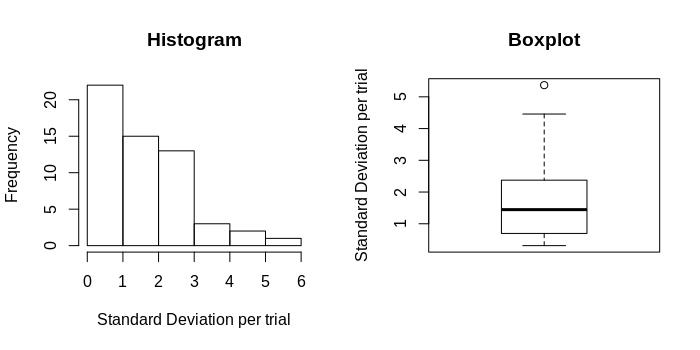
\includegraphics[width=9cm]{reportTemplate/figures/variance.png}
\caption{Variance in the repeated trials} \label{fig:trial_variance}
\end{figure}

We aggregated the raw data by calculating the average energy consumption and standard deviation over the 15 repetitions of each trial. In the remaining graphs and results, we use the average energy consumption for each (cluttered and de-cluttered) subject over these 15 repetitions. First, we discuss the standard deviations (SDs) of the trials to understand if the data is influenced by external factors. Ideally, the SD for each trial should be low as each experiment run with the same subject and cluttering state should have a similar energy consumption in a non-corrupted experiment setting. 

\newpage

The variability of the trials is visualized in Figure \ref{fig:trial_variance}. In the histogram, we observe that most trials have an SD between 0 and 1. The second\-largest groups have an SD between 1 and 3. The remaining subjects have an SD between 4 and 6. From the box plot, we observe that most subjects have indeed small SDs. However, there are some outliers and subjects with a larger SD.

\subsection{Data Distribution}

\begin{figure}[h]
\centering
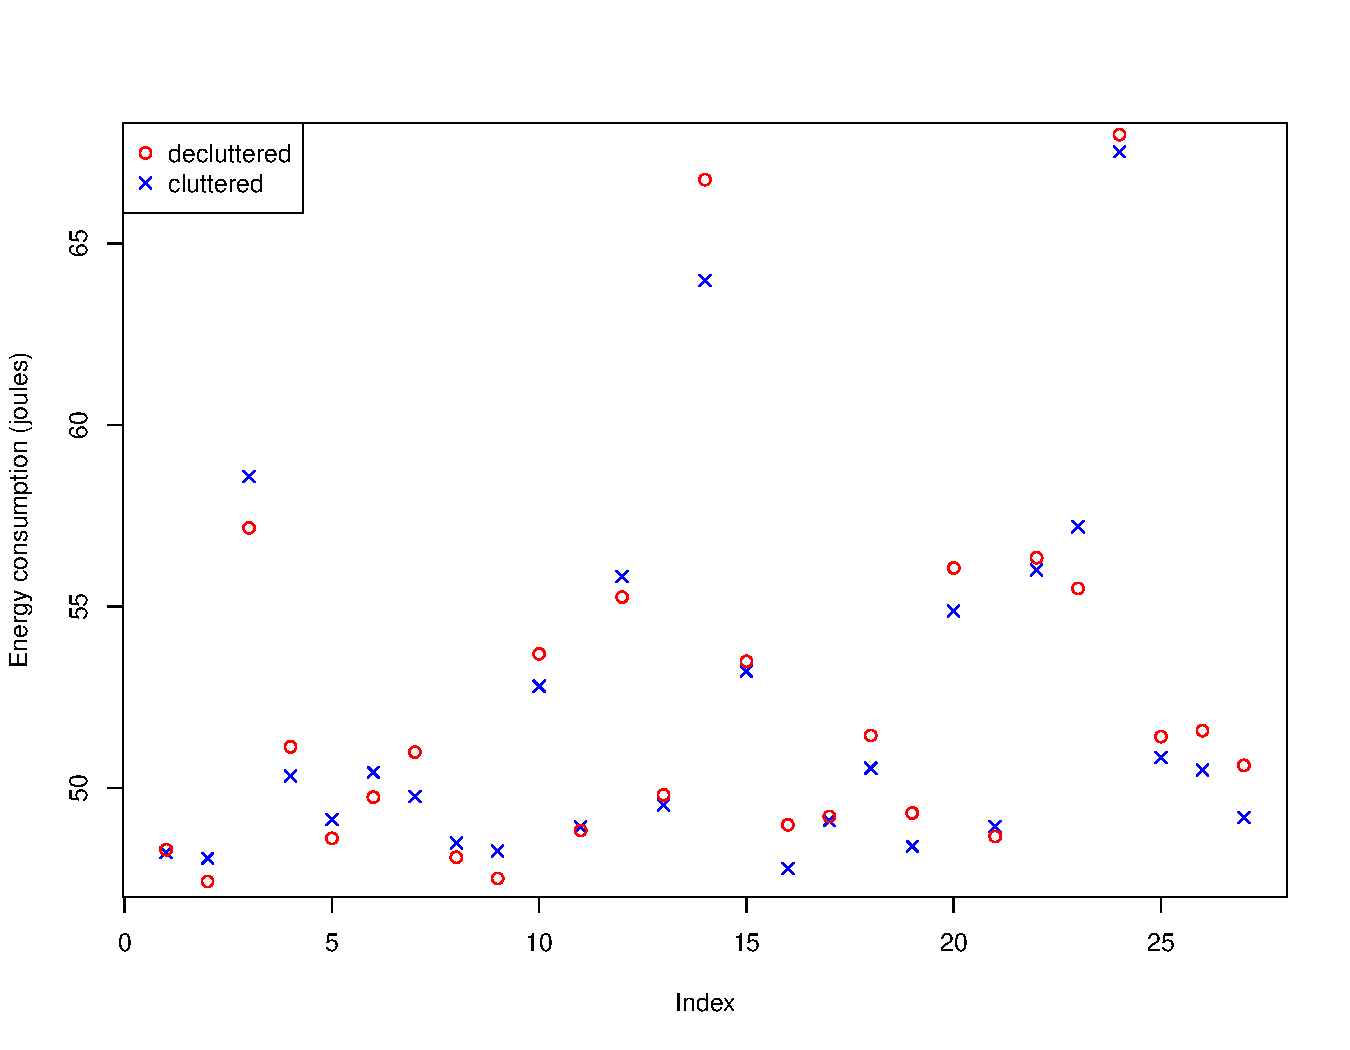
\includegraphics[width=9cm]{reportTemplate/figures/data_distribution/pl1.pdf}
\caption{Cluttered and de-cluttered joule measurements} \label{fig:clutter-declutter-data-all}
\end{figure}

Second, we present the data distributions of the average (over the 15 repetitions) energy consumption for each cluttered and de-cluttered mobile web app. Figure \ref{fig:clutter-declutter-data-all} presents a scatter plot containing the energy measurement for all subjects. From this figure, we observe that the measurements of the de-cluttered mobile web apps are close to the measurements of the cluttered mobile web apps.

\begin{figure}[h]
\centering
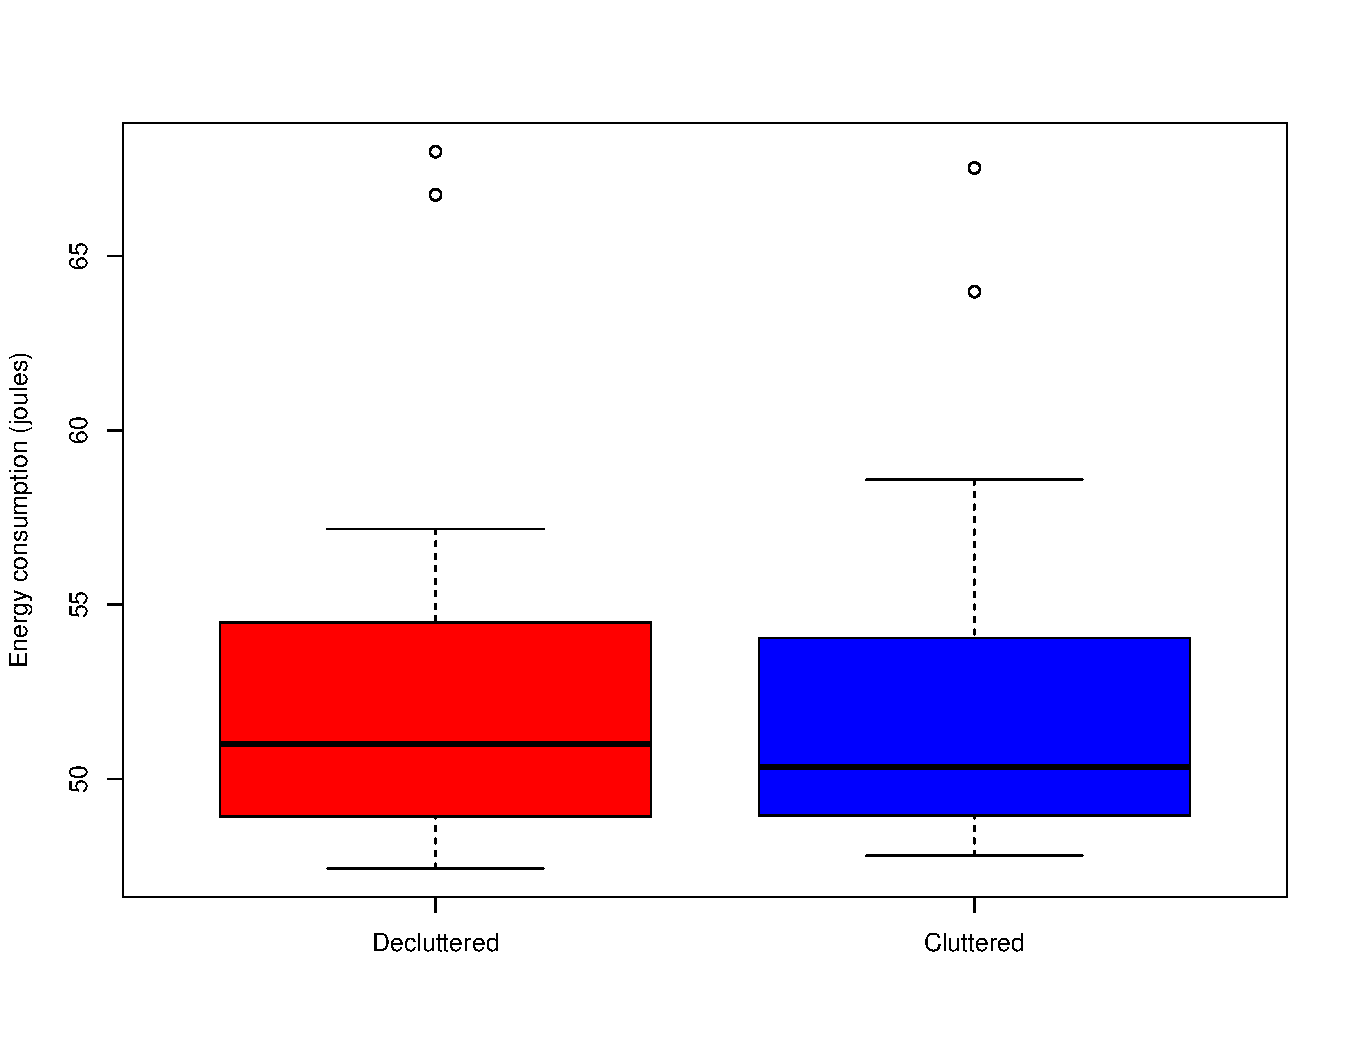
\includegraphics[width=9cm]{reportTemplate/figures/data_distribution/pl2.pdf}
\caption{Boxplot of the energy consumption for cluttered and de-cluttered mobile web apps} \label{fig:boxplot-clutter-vs-declutter}
\end{figure}

\begin{figure}[h]
\centering
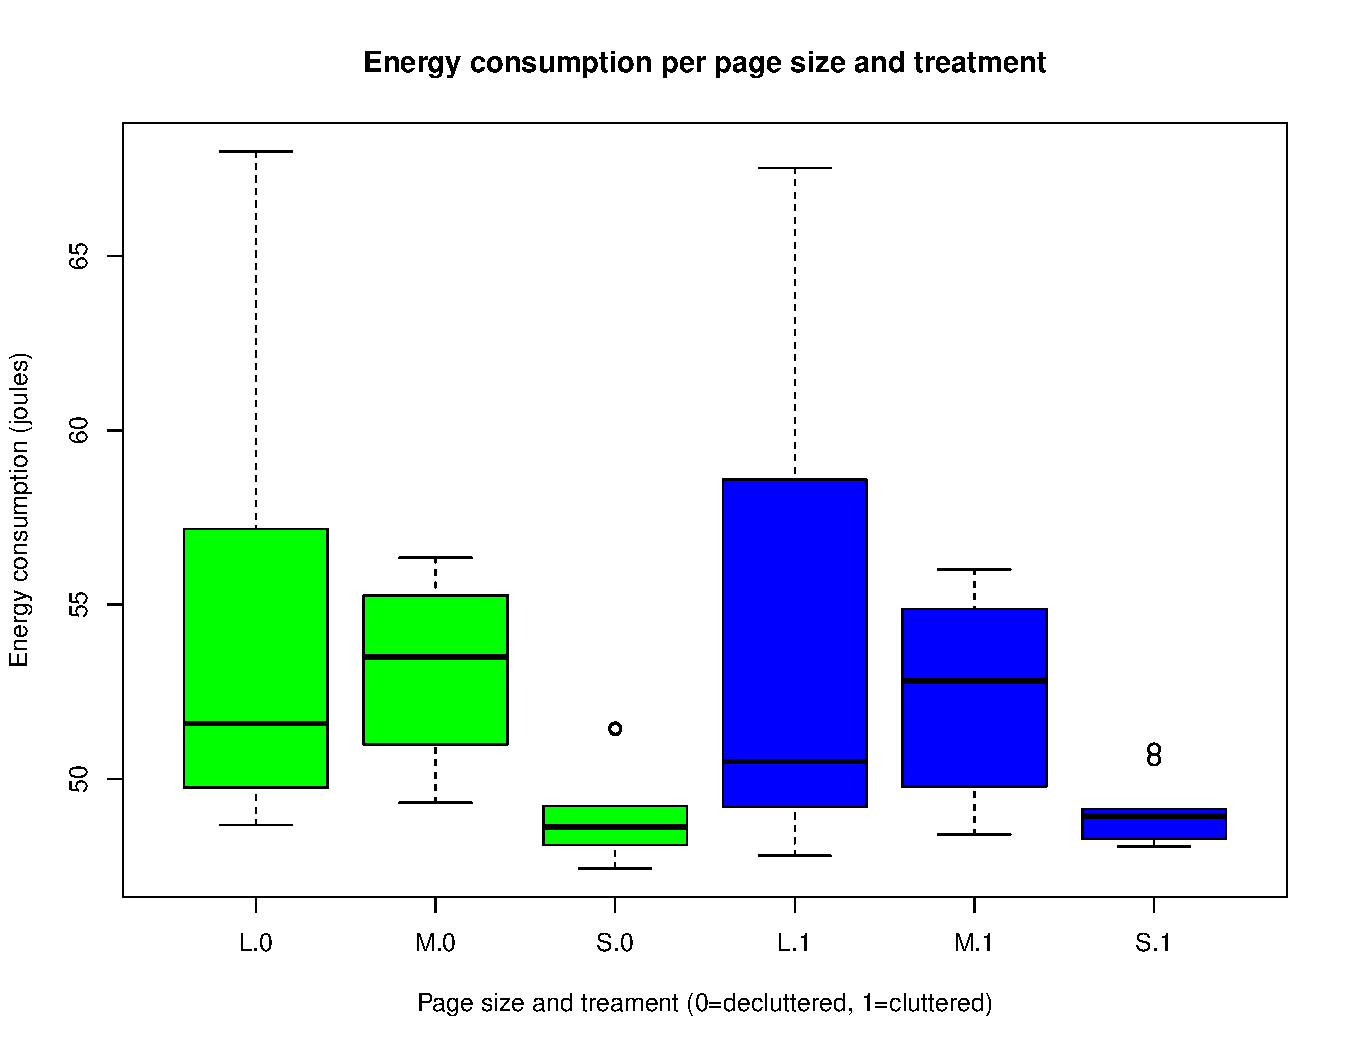
\includegraphics[width=9cm]{reportTemplate/figures/data_distribution/pl3.pdf}
\caption{Boxplot of the energy consumption for cluttered and de-cluttered mobile web apps, blocked into three page size classes} \label{fig:boxplot-clutter-vs-declutter-3-size-classes}
\end{figure}

\newpage
Next, from the box plot in Figure \ref{fig:boxplot-clutter-vs-declutter} we observe that the mean energy consumption of the cluttered treatment is lower than the mean energy consumption of the de-cluttered treatment. This gives an indication that the de-cluttered mobile web apps do not have a smaller energy consumption, without taking into account the page size. To further visually analyze the difference between the two treatments, we take into account the page size and visualize this in Figure \ref{fig:boxplot-clutter-vs-declutter-3-size-classes}. We observe that the smallest page size has indeed the smallest mean energy consumption for both treatments. This is expected as a small mobile web app takes fewer system resources to load compared to larger mobile web apps. However, medium-sized mobile web pages break this pattern as, for both treatments, we observe that the medium page size has a higher mean energy consumption compared to the pages in the `Large' category. 

\subsection{Testing Normality}

\begin{figure}[h]
\centering
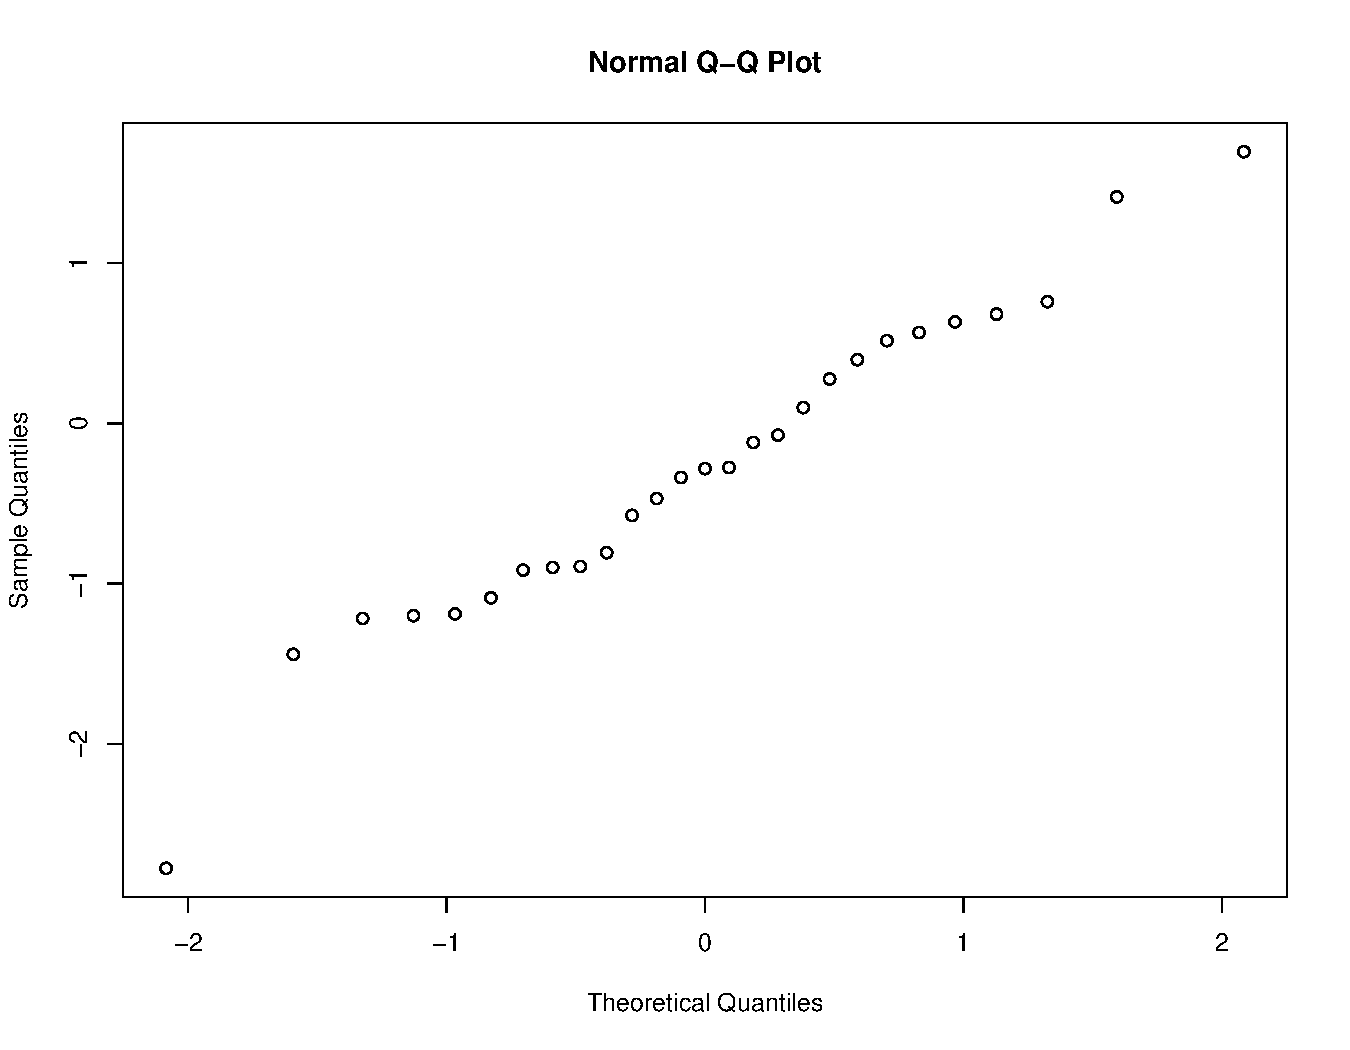
\includegraphics[width=9cm]{reportTemplate/figures/data_distribution/pl4.pdf}
\caption{Q-Q Plot of the difference between the cluttered and de-cluttered results} \label{fig:qq-plot-difference}
\end{figure}

Following the visualizations we test whether the data is normally distributed to determine which test is appropriate. In addition, we check if the difference between the treatments is normally distributed. This is required as a paired t-test is only applicable to data coming from a normal distribution. To execute these normality tests, we used the Shapiro-Wilk normality test. From this, we found a p-value of $0.746$, from which we conclude that the data is normally distributed. However, because the sample is quite small (27) and the Shapiro-Wilk test has a limited accuracy on a small sample size, we also perform a visual inspection using a Q-Q Plot. This plot is shown in Figure~\ref{fig:qq-plot-difference}. From this plot, we observe that the data is indeed approximately normally distributed as the data follows the diagonal line. This allows us to perform the paired t-tests.

\subsection{Paired t-tests}

Finally, we evaluated our hypothesis by executing paired t-tests on the observed data. First, we test whether the cluttered treatment has a significantly different mean compared to the de-cluttered treatment, without taking the page size into account. This test result is a p-value of $0.1472$. Using the significance level $\alpha$ of $0.05$ we conclude that without taking the page size into account, there is no significant difference in the energy consumption between the two treatments. Next, to test whether the treatment matters for the different page sizes, we run a paired t-test for each page individual page size category. From this, we find the following p-values: $0.6699$, $0.01402$, and $0.5268$ for the small, medium, and large page size categories respectively. Using the p threshold of $\frac{0.05}{3} = 0.016$, which is determined by the Bonferroni correction, we conclude that all three are insignificant. As the results are insignificant the effect size is irrelevant.
\section{Discussion}
Report implications and interpretations of your results (possibly grouped by research question).

\textcolor{red}{Page limit: 1}

\section{Threats To Validity}\label{sec:threats}
Report about each type of threat to the validity of the experiment, according to the classification discussed in class.

\subsection{Internal Validity}
\subsection{External Validity}
\subsection{Construct Validity}
\subsection{Conclusion Validity}

\textcolor{red}{Page limit: 1}


\section{Conclusions}\label{sec:conclusions}

% One brief paragraph for summarizing the main findings of the report.
In this study, we analyzed the energy consumption of cluttered JS code in mobile web apps. To do so, we randomly selected 27 subjects from the majestic million set. The subjects were de-cluttered using JSCleaner \cite{chaqfeh2020jscleaner}. We utilized Android Runner \cite{malavolta2020runner} to orchestrate and manage the experiment, and the Batterystats profiler to measure the energy consumption. Furthermore, we used statistical tests to conclude whether there is a significant difference in the energy consumption of the cluttered and de-cluttered mobile web apps. From these tests, no significant difference was found between the energy consumption of the cluttered and de-cluttered mobile web apps. This implies that developers do not need to take the energy consumption into account when applying a de-cluttering engine to their code. Considering that we used a small sample size to perform our experiments and tested solely one de-cluttering algorithm (JSCleaner), future studies are required to support this claim. %

% One brief paragraph about the possible extensions of the performed experiment (imagine that other 3 teams will be assigned to the extension of your experiment).
Future work could analyze a more extensive set of mobile web apps. Furthermore, the experiments could be performed on more devices (e.g. low- and high-end), operating systems (e.g. both iOS and Android), and browsers (e.g. Chrome, Firefox, Safari). Experiments done using these additions could substantiate the generalizability of the results and conclusions. In addition, more de-cluttering methods should be applied to the mobile web apps to test the difference between the effectiveness of the de-cluttering methods.

% Possible Extensions:
% 1. More samples
% 2. Real world setting
% 3. More devices
% 4. Apply more/other Cleaning methods
 

\bibliographystyle{IEEEtran}
\bibliography{references}

\end{document}
